\chapter{Introduction}\label{ch:intro}

\def \path {intro}
\def \imgpath {\path/images}

It has long been the goal of computer vision researchers to be able to develop
systems that can reliably recognize objects in a scene. Achieving this unlocks a huge
range of applications that can benefit society as a whole. From fully
autonomous vehicles, to automatic labelling of uploaded videos/images for searching,
or facial recognition for identification and security, the uses are far
reaching and extremely valuable. The challenge does not lie in finding the
right application, but in the difficulty of training a computer to \emph{see}.

There are nuisance variables such as changes in
lighting condition, changes in viewpoint and background clutter that do not
affect the scene but drastically change the pixel representation of it. 
Humans, even at early stages of their lives, have little difficulty filtering
these out and extracting the necessary amount of information from a scene. So
to design a robust system, it makes sense to design it off how \emph{our}
brains see. 

Unfortunately, vision is a particularly complex system to understand. It has
more to it than the simply collecting photons in the eye.
An excerpt from a recent Neurology paper \cite{raichle_two_2010} sums up the problem
well:

\begin{quotation}
It might surprise some to learn that visual information is significantly
degraded as it passes from the eye to the visual cortex. Thus, of the unlimited
information available from the environment, only about $10^{10}$ bits/sec are
deposited in the retina \ldots\ only $\sim 6\times 10^6$
bits/sec leave the retina and only $10^4$ make it to layer IV of V1
\cite{anderson_directed_2005,tor_norretranders_user_1998}. These data
clearly leave the impression that visual cortex receives an impoverished
representation of the world \ldots\ it should be noted that estimates of the
bandwidth of conscious awareness itself (i.e.,\ what we `see') are in the range
of 100 bits/sec or less\cite{anderson_directed_2005,
tor_norretranders_user_1998}.
\end{quotation}

Current digital cameras somewhat act as a combination of the first and second
stage of this system, collecting photons in photosensitive sensors and then
converting this to an image on the order of magnitude of $10^6$ pixels (slightly
larger but comparable to the $10^6$ bits/sec travelling through the optic
nerve).

If we are to build effective vision systems, it makes sense to emulate this
compression of information.
The question now stands before us --- what information is kept on entry to the V1 cortex?
Hubel and Wiesel revolutionized our understanding of the V1 cortex in the 50s and 60s by 
studying cats \cite{hubel_receptive_1959, hubel_receptive_1962}, macaques and spider 
monkeys \cite{hubel_receptive_1968}. They found that neurons in the V1 cortex fired
most strongly when edges of a particular (i.e.,\ neuron-dependent) orientation
were presented to the animal, so long as the edge was inside the receptive field of
this neuron.
Continued work on their experiments by Blakemore and Cooper
\cite{blakemore_development_1970} showed, by exposing
kittens to controlled environments in which they only saw horizontal and
vertical lines, that these early layers of perception are in fact \emph{learned}. 
% A figure of the the frequency response of the photoreceptor cells in our eyes
% to different wavelengths of light.
% \begin{figure}
  % \begin{center}
      % 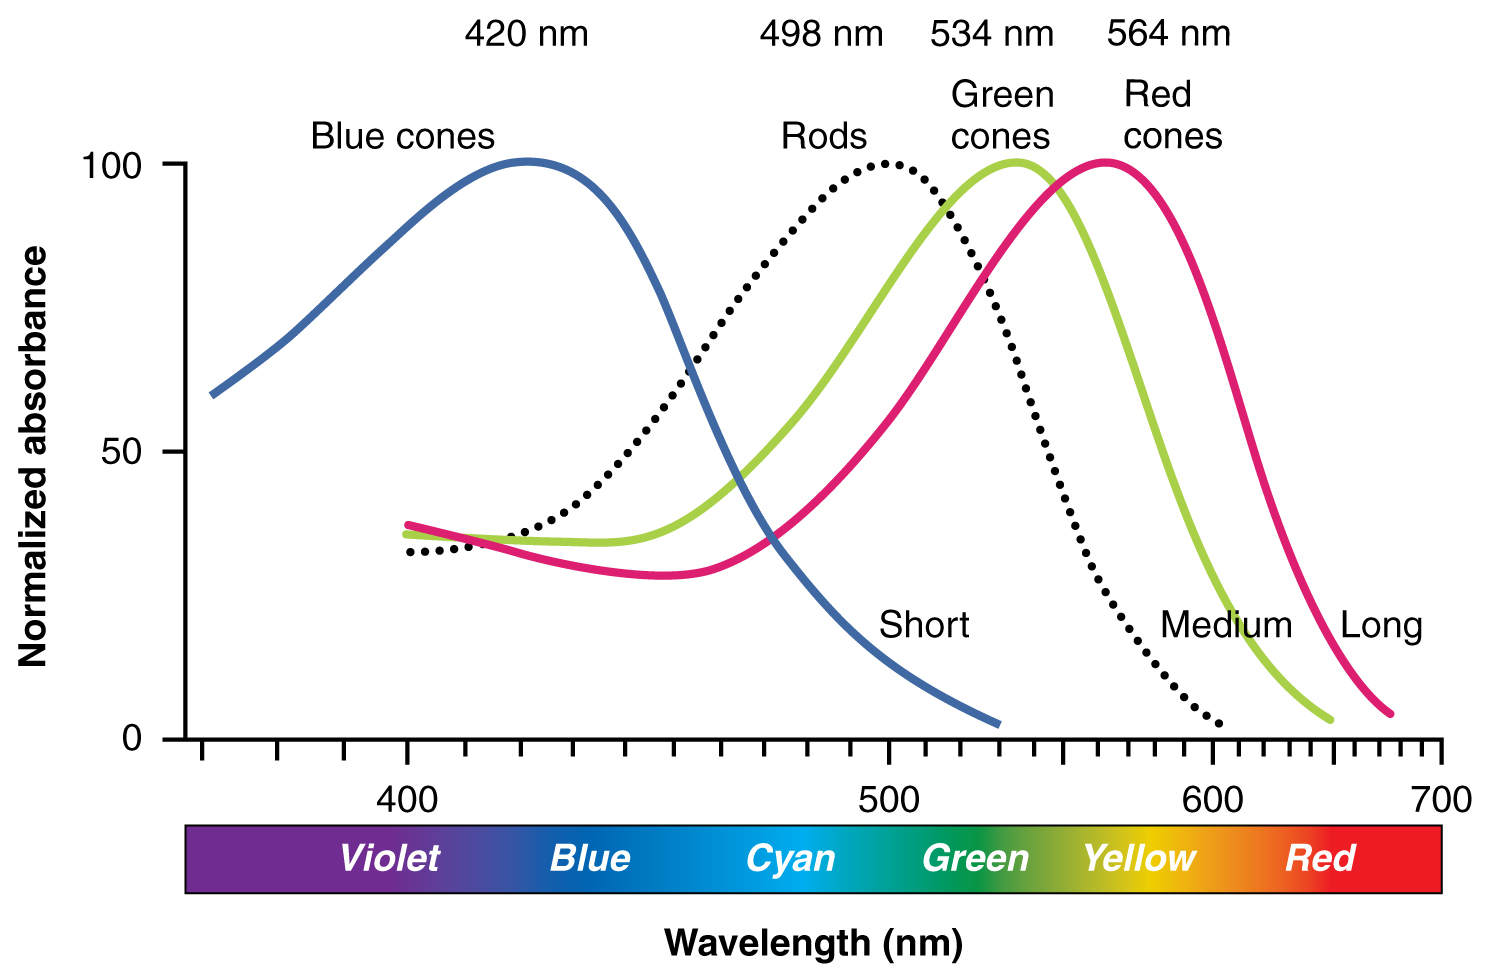
\includegraphics[width=10cm]{\imgpath/colour_sensitivity.jpg}
      % \mycaption{Frequency sensitivity of photoreceptors in they eye}
              % {Wavelength responsiveness of the different photoreceptors in the
               % eye. S, M, and L are short, medium, and long cones, compared to
               % R --- rods. Taken from~\cite{bowmaker_visual_1980}}
  % \end{center}
% \end{figure}

\section{Convolutional Neural Networks}
  \begin{figure}
    \centering
      % \includegraphics[width=\textwidth]{\imgpath/dtcwt_gain}
      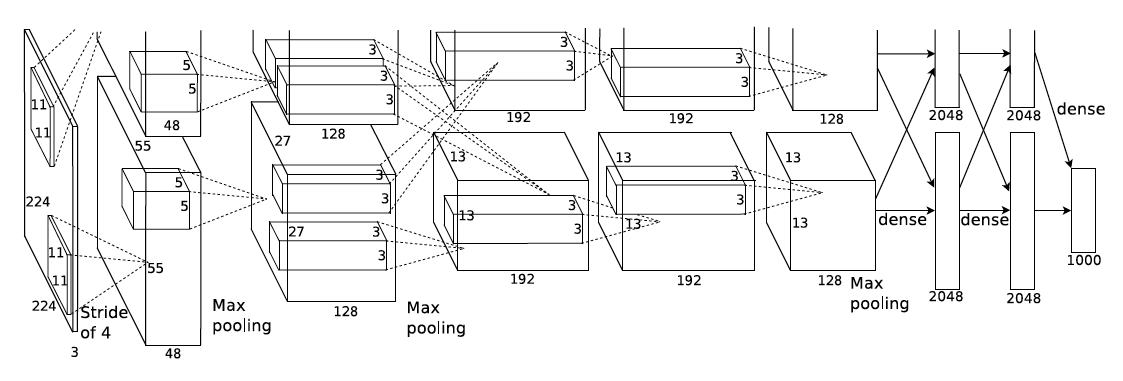
\includegraphics[width=\textwidth]{\imgpath/alexnet.png}
      \mycaption{Convolutional Architecture of
      \cite{krizhevsky_imagenet_2012}}{}
      \label{fig:ch1:cnn_arch}
    \end{figure}
The current state of the art in image understanding sysems are 
Convolutional Neural Networks (CNNs). These are a learned model that
stacks many convolutional filters on top of each other separated by
nonlinearities. 
They are seemingly inspired by the visual cortex in the way that they are
hierarchically connected, progressively compressing the information into a
richer representation. 

\autoref{fig:ch1:cnn_arch} shows an example 
architecture for the famous AlexNet \cite{krizhevsky_imagenet_2012}. Inputs are resized to a
manageable size, in this case $224\x 224$ pixels. Then multiple convolutional
filters of size $11\x 11$ are convolved over this input to give $96$ output
\emph{channels} (or \emph{activation maps}). In the figure, these are split onto two 
graphics cards or GPUs for memory purposes. These are then passed through a
a pointwise nonlinear function, or a \emph{nonlinearity}.
The activations are then pooled (a form of downsampling) and convolved with more
filters to give $256$ new channels at the second stage. This is repeated 3 more
times until the $13\x 13$ output with $256$ channels is unravelled and passed
through a fully connected neural network to classify the image as one of $1000$
possible classes.
  
CNNs have garnered lots of attention since 2012 when the previously mentioned AlexNet
nearly halved the top-5 classification error rate (from $26\%$ to $16\%$) 
on the ImageNet Large Scale Visual Recognition Competition (ILSVRC)
\cite{russakovsky_imagenet_2014}\footnote{The previous state of
the art classifiers had been built by combining keypoint extractors like 
SIFT\cite{lowe_distinctive_2004} and HOG\cite{dalal_histograms_2005} with
classifiers such as Support Vector Machines\cite{cortes_support-vector_1995} and
Fisher Vectors\cite{sanchez_image_2013}, for example \cite{sanchez_high-dimensional_2011}.}.
In the years since then, their complexity has grown significantly. AlexNet had
only 5 conovlutional layers, whereas the 2015 ILSVRC winner ResNet \cite{he_deep_2016}
achieved 3.57\% top-5 error with 151 convolutional layers (and had some
experiments with 1000 layer networks).

\section{Problems with CNNs and Project Motivation}\label{sec:motivation}
\begin{figure}
  \centering
  \subfloat[conv1 filters]{
  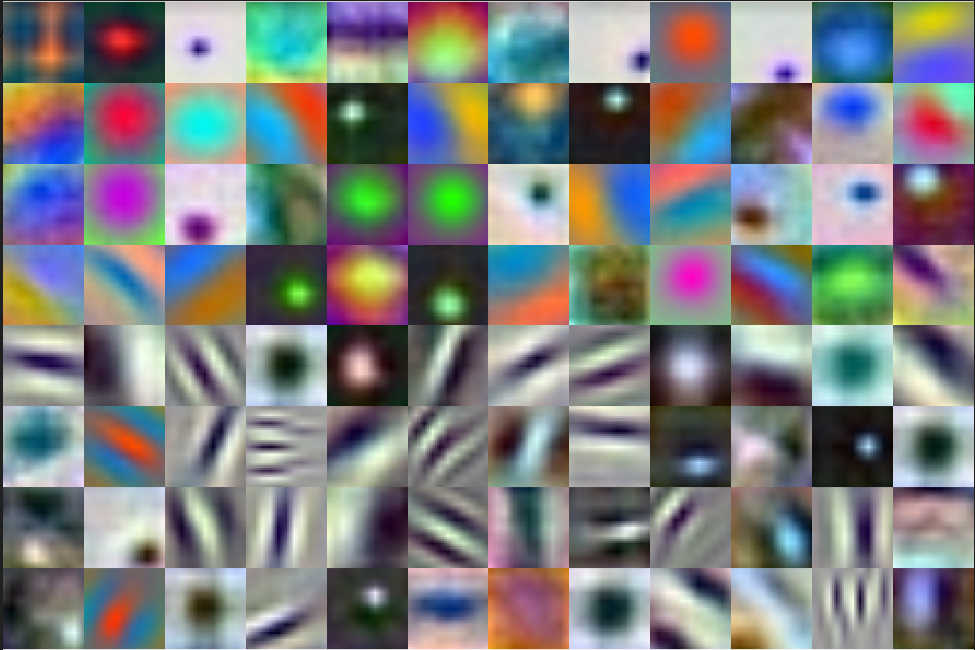
\includegraphics[width=0.6\textwidth]{\imgpath/alexfilters.png}
  \label{fig:ch1:alex_filt}
  }\\
  \subfloat[conv1 activations]{
  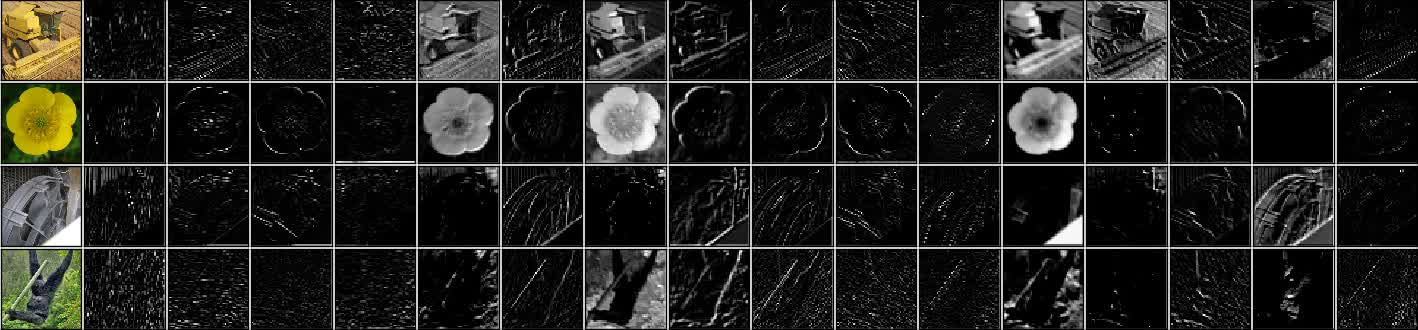
\includegraphics[width=\textwidth]{\imgpath/out1.jpg}
  \label{fig:ch1:alex_conv1}
  }\\
  \subfloat[conv2 activations]{
  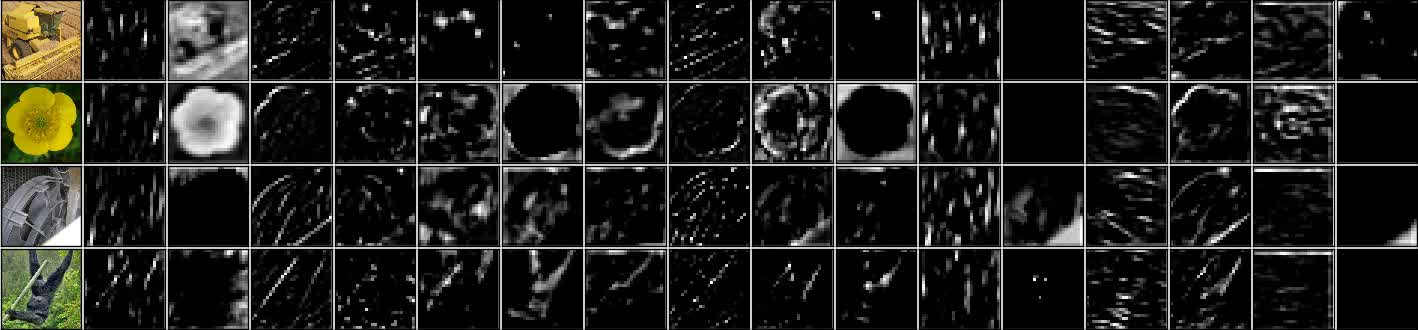
\includegraphics[width=\textwidth]{\imgpath/out2.jpg}
  \label{fig:ch1:alex_conv2}
  }\\
  \subfloat[conv3 activations]{
  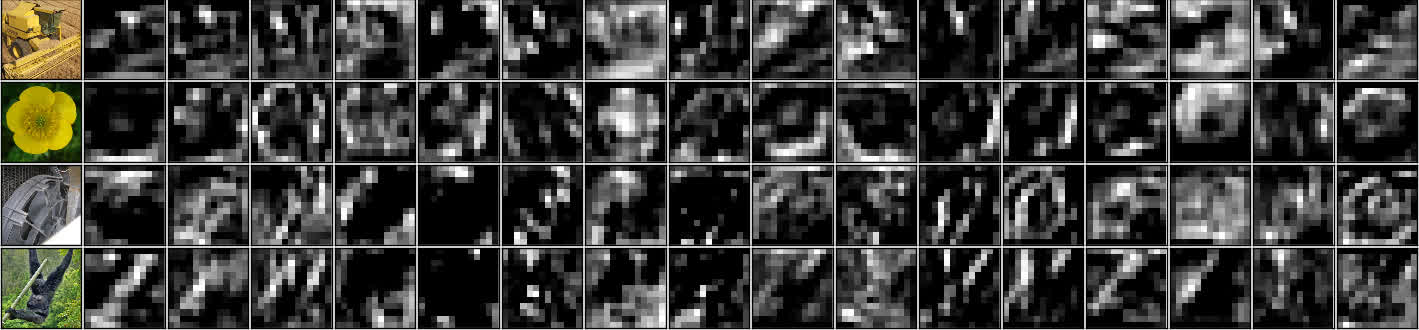
\includegraphics[width=\textwidth]{\imgpath/out3.jpg}
  \label{fig:ch1:alex_conv3}
  }
  \mycaption{The first layer filters learned by AlexNet and the first three
  layer's activations}{\subref{fig:ch1:alex_filt} The $11\x 11$ filters for the
  first stage of AlexNet. Of the 96 filters, 48 were learned on one GPU and
  another 48 on another GPU. Interestingly, one GPU has learned mostly
  lowpass/colour filters and the other has learned oriented bandpass
  filters. \subref{fig:ch1:alex_conv1} - \subref{fig:ch1:alex_conv3} Randomly
  chosen activations from the output of the first, second and third convolutional 
  layers of AlexNet (see \autoref{fig:ch1:cnn_arch}) with negative values set to 0. 
  Filters and activation images taken from supplementary material of
    \cite{krizhevsky_imagenet_2012}.}
  \label{fig:ch1:alexnet_filters}
\end{figure}
Despite their success, they are often criticized for being \emph{black box}
methods. You can view the first layer of filters
quite easily (see \autoref{fig:ch1:alex_filt}) as they exist in RGB
space, but beyond that things get trickier as the filters have a third, \emph{depth}
dimension typically much larger than its two spatial dimensions. Additionally,
it is not clear what the input channels themselves correspond to. For illustration
purposes, we have also shown some example activations from the first three
convolutional layers for AlexNet in
\autoref{fig:ch1:alex_conv1}-\autoref{fig:ch1:alex_conv3}. These activations are
taken after a specific nonlinearity that sets negative values to 0 (hence the
large black regions). We can see in `conv1' (\autoref{fig:ch1:alex_conv1}) that
some of the first layer channels are responding to edges or colour information,
but as we go \emph{deeper}, it becomes less and less clear
what each activation is responding to.

Aside from their lack of interpretability, it takes a long time and a lot of
effort to train state of the art CNNs. Typical networks that have won ILSVRC
since 2012 have had roughly 100 million parameters and take up to a week to train. This 
is optimistic and assumes that you already know the necessary optimization or
architecture hyperparameters, which you often have to find out by trial and error. 
In a conversation the author had with Yann LeCun, the attributed father of
CNNs, at a Computer Vision Summer School (ICVSS), LeCun highlighted this problem
himself:
\begin{quote}
  There are certain recipes (for building CNNs) that work and certain recipes
  that don't, and we don't know why.
\end{quote}

Considering the recent success of CNNs, it is becoming more and more
important to understand \emph{how} and \emph{what} a network learns, which
has contributed to it making its classification or regression choice.
Without this information, the use of these incredibly powerful tools could be
restricted to research and proprietary applications.

They are fairly crude in terms of signal processing, as
the filters are arbitrary FIR filters. It is important to find ways to find an
adequate richness to the filtering. It must still be large yet the number of the
parameters needed to specify this should be kept as small as possible.

  In particular, the starting point for our project is clear --- the filters
  learned by the first layer of a CNN, shown in
  \autoref{fig:alexnet_filters},
  look like oriented wavelets. This is not surprising either from a biological
  point of view --- as it matches the earlier mentioned results by Hubel and
  Wiesel, or from a signal processing point of view --- as the wavelet
  transform is a powerful and stable way to split up an image into areas of the
  frequency domain.
  
  % Attempts have been made in the past to enhance a system that detects edges
  % into a system that can detect the next level in the hierarchy --- corners
  % and curves. This is a particularly difficult task to do without learning,
  % due to the very large number of permutations each corner can come in. 

  With this, the above goal can then be refined to a more targeted one:

  %\begin{minipage}
  \newpage
  \begin{goals}\bf
    Starting with a wavelet transform, we want to look at how to develop
    a higher order system by drawing inspiration from the second and third
    layers of a CNN\@. Achieving this will shed light on what is learned and what
    is needed for a good image recognition system.
  \end{goals}
  %\end{minipage}

  The second inspiration for a starting point is the recent work in developing
  \emph{Scatternets} by Stephan\'{e} Mallat, one of the forefathers of the wavelet
  transform, and his research group. Their work attempts to do precisely
  what we want --- start with a wavelet transform that is sensitive to edges,
  and then build deeper layers on top of this that are sensitive to larger
  shapes, while being insensitive to uninformative variations such as
  translation, rotation, and scale. Their Scatternets are purely deterministic.

For example the evolution of the convolutional net over the MLP is a classic
example of how restriction led to improvement.


As an example\footnote{While we limit the scope of our project to Imaging
problems, CNNs can and have been used successfully in time series and
language tasks.}, it is not hard to imagine a deep network that could be used to
assess whether giving a bank loan to an applicant is a safe investment. It
could compare a vector of their current and past financial situation to
a dataset of others and choose a simple yes/no answer. Trusting a black box
solution is deeply unsatisfactory in this situation. Not only from the
customer's perspective, who, if declined, has the right to know why
\cite{goodman_european_2016}, but
also from the bank's --- before lending large sums of money, most banks
would like to know why the network has given the all clear. `It has worked well
before' is a poor rule to live by.

  We are not the first research group to be unsatisfied with not knowing the
  mechanics of CNNs. There has been a lot of very impressive work done recently
  on trying to visualize the response a CNN has to a given input, in particular
  the work done by \cite{zeiler_visualizing_compact_2014}, which builds
  `Deconvolutional Neural Networks' (deconvnets) to view the regions of the
  input image that cause large responses at deeper layers of a CNN\@. This was the key
  tool in the previously mentioned `Why Should I Trust You?' paper
  \cite{ribeiro_why_2016} to find the regions of the image that make up
  \autoref{fig:interpretability}.

  So far these tools, while useful, stop short of turning visualization around into an
  improved strategy for designing networks. This brings us to the main goal of
  our research:

  \begin{goals}\bf
    We hope to further research into understanding \emph{how} and \emph{what} deep networks
    learn by building a well understood and well-defined network that mimics
    their operation. Intuition is the primary goal, and with that, we
    believe improved performance will follow.
  \end{goals}

  We do not wish to focus only on purely handcrafted methods, nor on purely
  learned methods. Neither is discounted, and a hybrid of the two seems to be
  a good way to achieve our goal. 

\section{Layout}
  The layout of the report is as follows.
  \autoref{ch:litreview} explores some of the background necessary for starting
  to develop image understanding models. In particular, it covers the
  inspiration for CNNs and the workings of CNNs themselves. 

  \autoref{ch:freq_analysis} covers the wavelet transform used by Mallat, and
  compares it to the preferred Dual-Tree Complex Wavelet Transform (\DTCWT) by
  Kingsbury \cite{kingsbury_complex_2001}.

  \autoref{ch:scatternets} reviews in depth the Scatternet designs by Mallat
  et.\ al.
  This is the last chapter of literature review, before
  \autoref{ch:dtcwt_scatternets} which starts to explore our work and analysis
  done on these Scatternets. In particular, we swap out the Morlet wavelets from
  Mallat's Scatternet to the faster, separable \DTCWT\
  wavelets, but we also make changes to the design of the Scatternet and look at
  how to apply the principles of visualizations, like those in the work by
  \cite{zeiler_visualizing_compact_2014}.

  \autoref{ch:scat_deep} then explores our recent work in attempting to combine
  Scatternets with CNNs. The inspiration for this being the idea that
  a well designed tool like the Scatternet, followed by a shallower CNN, should
  be equivalent to or better than a deeper CNN.

  \autoref{ch:conclusion} then summarizes our findings so far, discusses and
  analyses the results, and lays out the plan for the remainder of the project.
  

This work is stimulated by the intuition that wavelet decompositions, in particular
complex wavelet transforms, are good building blocks for doing image recognition
tasks. Their well understood and well defined behaviour as well as the
similarities seen in learned networks, implies that there is potential gain for
thinking about CNN layers in a new light. 

To explore and test this intuition, we begin by looking at one of the most popular current uses of
wavelets in image recognition tasks, in particular the Scattering Transform. 

\section{Series Expansions of Signals}
Look at the intro to Vetterli's book. Want to make a statement about expanding
signals in some form or another.

\section{Contributions}
The contributions and layout of this thesis are:

\begin{itemize}
  \item \textbf{Software for wavelets and $\DTCWT$ based ScatterNet (chapter 3)}
  \item \textbf{ScatterNet analysis and visualizations (chapter 4)}. Presented
    at MLSP2017, this chapter 
  \item \textbf{Invariant Layer/Learnable ScatterNet (chapter 5)} Presenting at
    ICIP2019.
  \item \textbf{Learning convolutions in the wavelet domain (chapter 6)}.
\end{itemize}

\subsection{Desirable Properties}
Unlike CNNs introduced earlier which have little prior constraints (apart
from the commonly used $L_2$ regularization), the scattering operator may be 
thought of as an operator $S$ that imposes structural priors on learning by
extracting features with manually chosen, desirable properties. The extracted
features can be used In classical
paradigms of image understanding, it makes sense to add these priors, but it
remains yet to be shown that these help learning.

limit variability these properties areview on these
properties are manually chosen with the ultimate goal of aiding image
understanding. 

